%\begin{figure}
\begin{center}
\tikzstyle{hidden}=[circle,
                        thick,
                        draw=black,
                        fill=white]
                        % minimum size=1.5ex,


\tikzstyle{observed}=[circle,
                        thick,
                        draw=black,
                        fill=gray!60]
                        % minimum size=1.5ex,


\tikzstyle{plate}=[rectangle,
                        draw=black,
                        fill=none,
                        inner sep=.8ex,
                        rounded corners=.6ex]

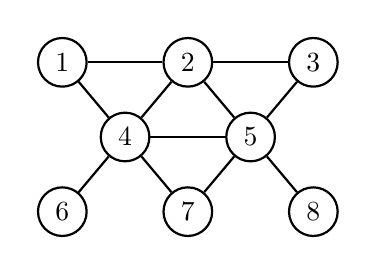
\begin{tikzpicture}[>=latex] %,text height=1.5ex,text depth=0.25ex]
  \matrix[row sep=2ex,column sep=1ex] {
        \node (1) [hidden] {$1$};  & &
        \node (2) [hidden] {$2$};  & &
        \node (3) [hidden] {$3$}; \\ &
        \node (4) [hidden] {$4$};  & &
        \node (5) [hidden] {$5$};  & \\
        \node (6) [hidden] {$6$};  & &
        \node (7) [hidden] {$7$};  & &
        \node (8) [hidden] {$8$}; \\
    };
    
    % The diagram elements are now connected through arrows:
    \path[-]
        (1) edge[thick] (4)
        (2) edge[thick] (4)
        (2) edge[thick] (5)
        (3) edge[thick] (5)
        (4) edge[thick] (6)
        (4) edge[thick] (7)
        (5) edge[thick] (7)
        (5) edge[thick] (8)
        (1) edge[thick] (2)
        (2) edge[thick] (3)
        (4) edge[thick] (5)
;
        
\end{tikzpicture}
\end{center}
%\caption{}
%\end{figure}